\chapter{Диаграммы}
\label{cha:appendix1}

\begin{figure}
  \centering
  \includegraphics[scale=0.9]{inc/svg/complexDeploy}
  \caption{Схема развертывания AEM среды}
  \label{fig:complexDeploy}
\end{figure}

\begin{figure}
  \centering
  \includegraphics[width=\textwidth]{inc/img/handler1}
  \caption{Конфигурация 1 SAML 2.0 Authentication Handler}
  \label{fig:defaultHandlerConfig1}
\end{figure}

\begin{figure}
  \centering
  \includegraphics[width=\textwidth]{inc/img/handler2}
  \caption{Конфигурация 2 SAML 2.0 Authentication Handler}
  \label{fig:defaultHandlerConfig2}
\end{figure}

\begin{figure}
  \centering
  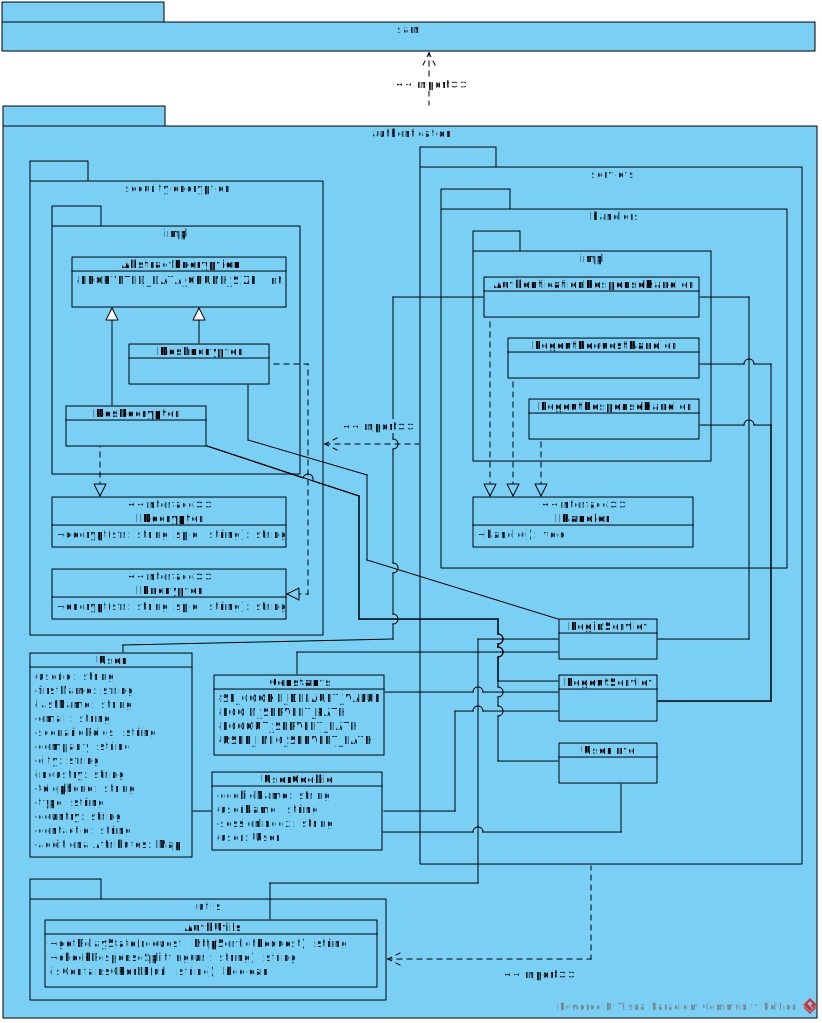
\includegraphics[width=\textwidth]{inc/svg/authenticationModule}
  \caption{Диаграмма классов пакета authentication}
  \label{fig:authenticationModule}
\end{figure}

\begin{figure}
  \centering
  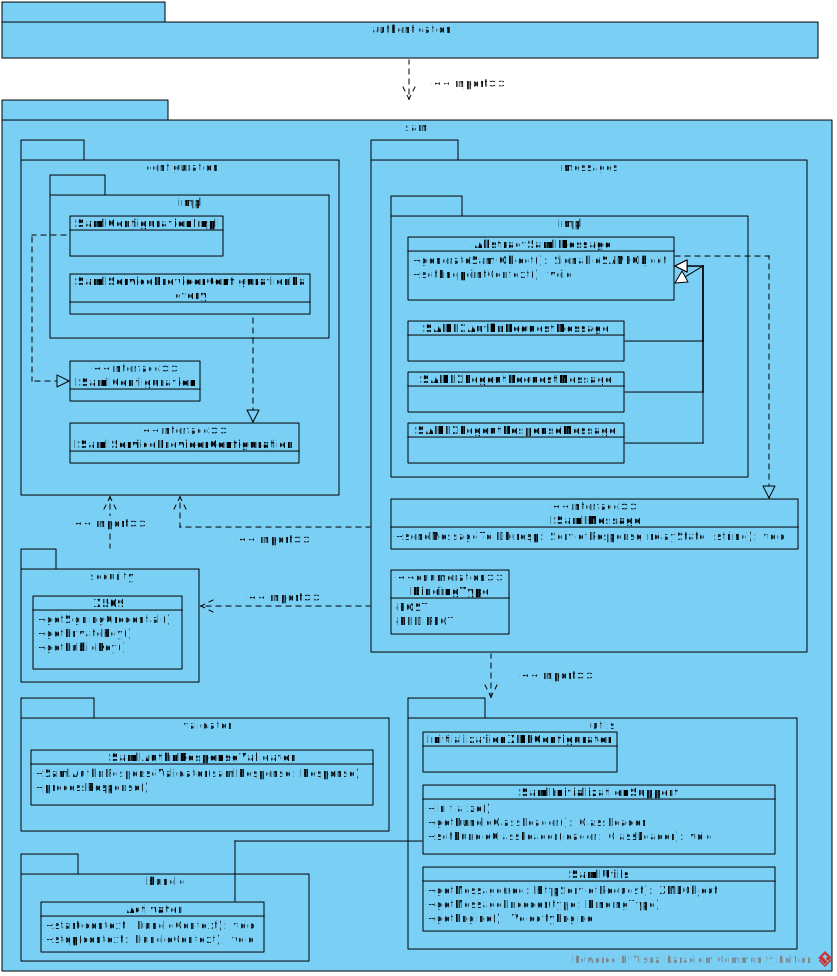
\includegraphics[width=\textwidth]{inc/svg/samlModule}
  \caption{Диаграмма классов пакета saml}
  \label{fig:samlModule}
\end{figure}

\begin{listing}[H]
\inputminted[linenos,frame=single]{java}{inc/src/SamlInitializationSupport}
\caption{Класс инициализации Open SAML 3} 
\label{lst:samlInitialization}
\end{listing}

\begin{longlisting}
\inputminted[linenos,frame=single]{java}{inc/src/validation}
\caption{Код валидации полученного утверждения} 
\label{lst:validation}
\end{longlisting}

%%% Local Variables: 
%%% mode: latex
%%% TeX-master: "rpz"
%%% End: 
